\section{Компьютерная морфология}\label{sect_review_comp_morphology}

Морфология -- это раздел лингвистики, изучающий структуру слова и его грамматические значения~\cite{MitreninaNikolaevLando2016}. Другими словами, морфология изучает
1) часть речи,
2) словоизменение,
3) словообразование,
4) грамматическое значение (что слово означает в предложении).

Компьютерная морфология анализирует и синтезирует слова программными средствами~\cite{MitreninaNikolaevLando2016}.

В компьютерной морфологии взаимосвязаны три базовых понятия: лемма, граммема и словоформа.
\begin{enumerate}
    \item \emph{Лемма}~-- это базовая, каноническая форма слова.
        Например, инфинитив у глагола.

    \item Грамматическое значение представляется в виде набора \emph{граммем}.
        Граммему также называют грамматической характеристикой,
          морфологическим признаком, морфологическим свойством,
          тегом (при разметке текста).
        Граммемы группируются по категориям (падеж, время и т.~д.).
        Одна и та же форма слова не может иметь две граммемы одной категории
        (например, глагол не может иметь сразу форму прошлого и настоящего времени).
        С другой стороны, формы могут совпадать, и их нужно уметь различать.

    \item \emph{Словоформа}~-- это\ldots \TODO{TODO}
\end{enumerate}

\emph{Лингвистическа разметка}~--- это процесс или результат 
приписывания текстам и их компонентам специальных меток, 
позволяющих выполнять поиск по лингвистическому корпуса~\cite[415]{Kibrik2019}.
%
В корпусной лингвистике есть ряд требований к разметке, известных как 
семь максим Лича~\cite[415--416]{Kibrik2019}. 


\subsubsection{Морфологическое словоизменение и морфологический анализ}

Морфологическое словоизменение\footnote{%
    \emph{Морфологическое словоизменение} по-английски звучит как
    ``inflectional morphology''.
    \emph{Система} и \emph{задача морфологического словоизменения}
    будут переводиться как
    ``morphological inflection system'' и ``morphological inflection task'' соответственно,
    см. например, американскую статью~\cite{King2020seq2seqRussianMA}.
} или просто словоизменение~--
это отображение лемм и набора морфологических признаков
на соответствующую словоформу~\cite[2821]{Cruz-Anastasopoulos-Stump2020Chatino}.

Под \emph{морфологическим анализом} слова или словоформы (morphological analysis)
подразумевается определение леммы и
грамматических характеристик словоформы~\cite{MitreninaNikolaevLando2016}.

Таким образом, если задачу <<морфологического словоизменения>> обозначить как прямую
(по лемме и признаку нужно найти словоформу),
то <<морфологический анализ>> (по словоформе требуется найти
лемму и морфологические свойства) будет обратной задачей.

\begin{figure}
    \centering
    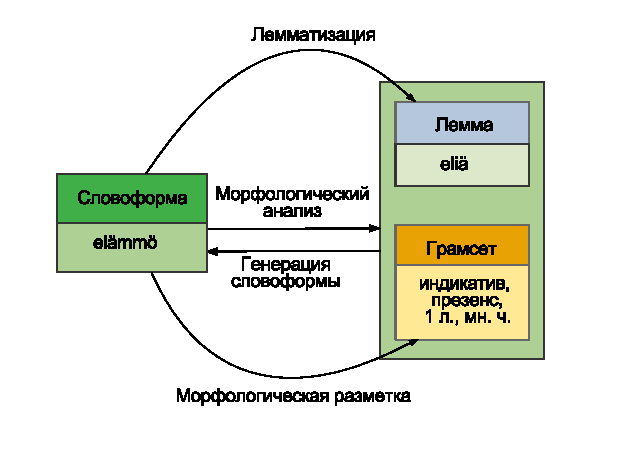
\includegraphics[width=0.75\textwidth,keepaspectratio=true]{inflectional_operations_v2}
%      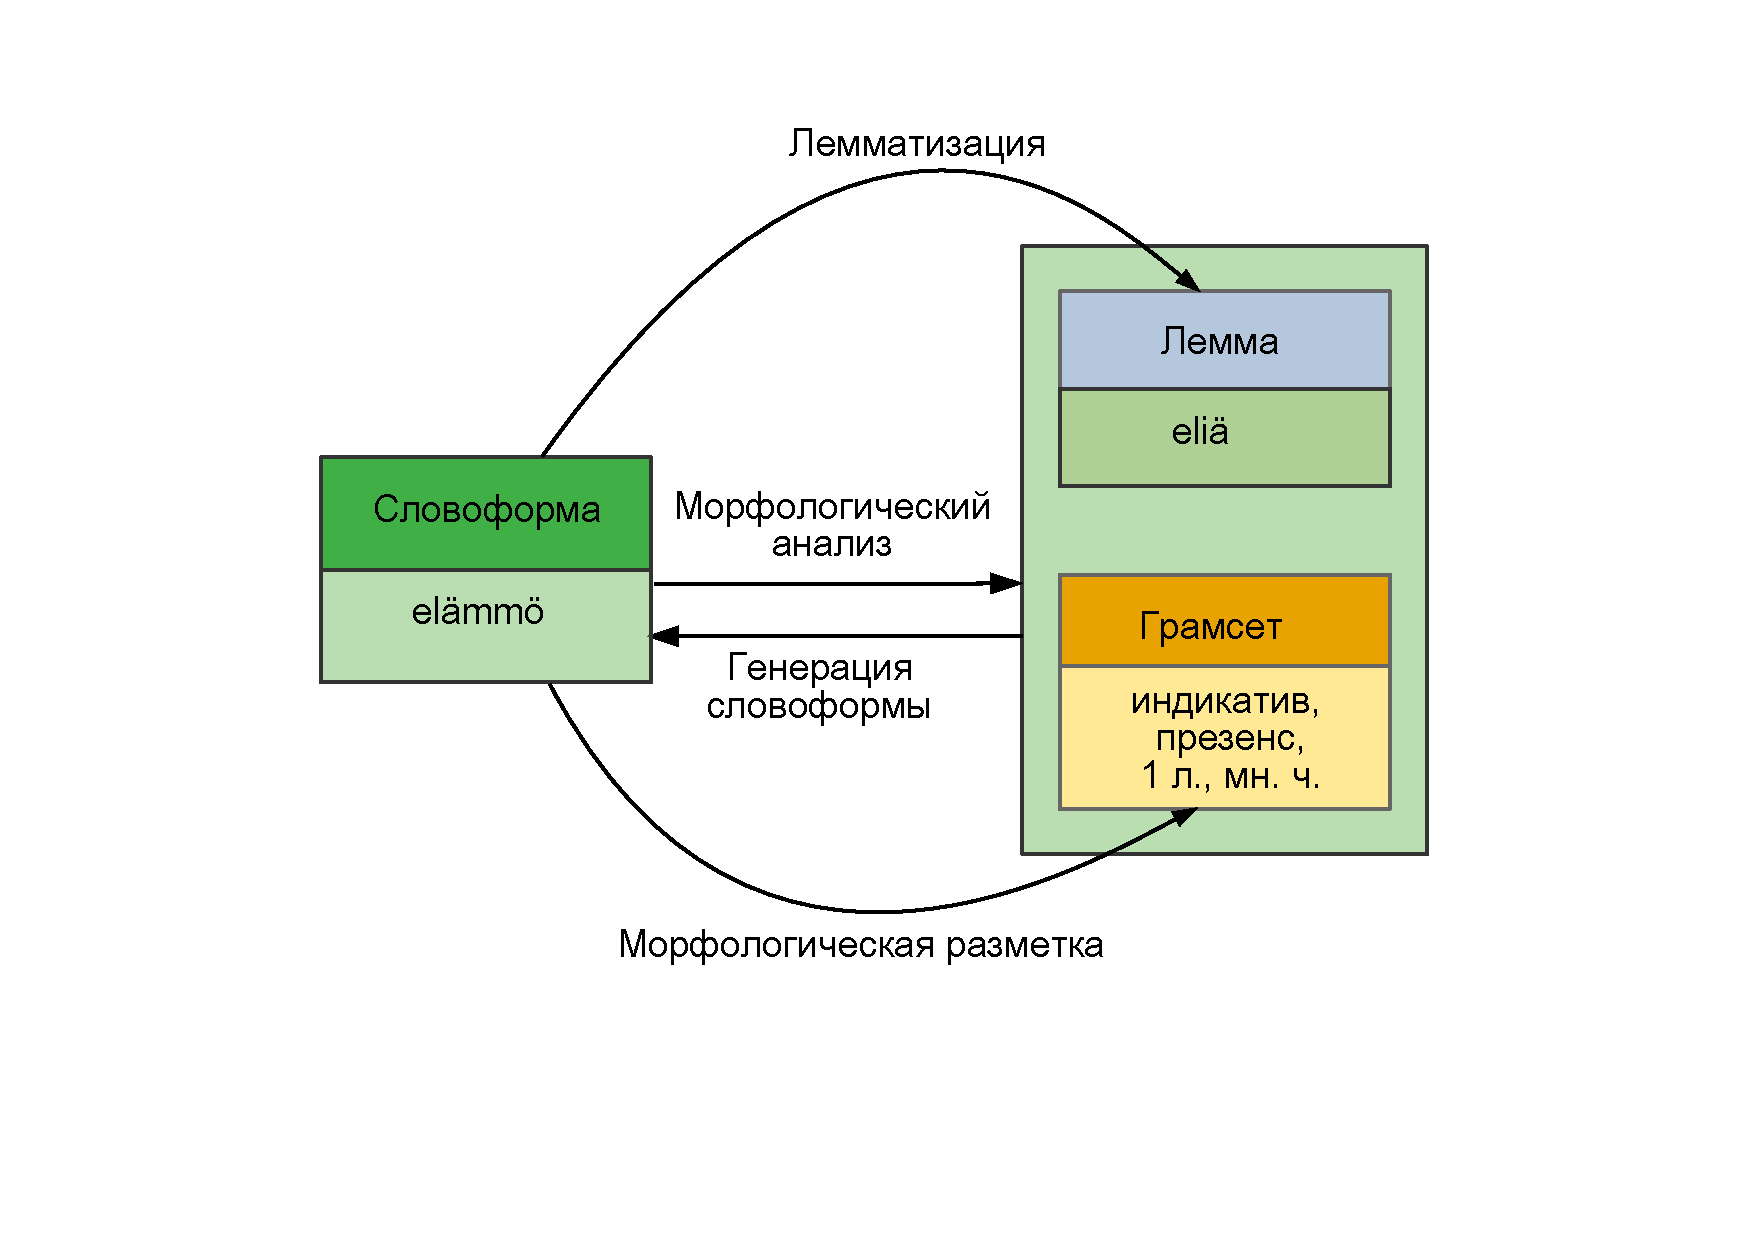
\includegraphics[width=1\linewidth]{inflectional_operations.pdf}
\caption{Четыре морфологические операции: генерация, анализ, лемматизация и разметка. Адаптация рисунка из статьи~\cite{Nicolai2020FineGraned}.} \label{fig:inflectional_operations}
\end{figure}

Отметим, что в ряде языков отсутствует морфологическое словоизменение,
например, в языках йоруба и севернокитайском~\cite[2]{Vylomova2020Sigmorphon}.




\subsubsection{Paradigm Cell Filling Problem}

С задачей морфологического анализа тесно связана задача
``a paradigm cell filling problem'' (PCFP)~\cite{Ackerman08PartsAndWholes}.



\subsubsection{Соревнования по морфологическому анализу (и результаты?)}

Рассмотренные выше задачи решают на соревнованиях
между компьютерными программами в рамках различных конференций:
\begin{description}[align=left]
    \item [Диалог]\footnote{См. \url{http://www.dialog-21.ru}}~--
            известная отечественная конференция
            по компьютерной лингвистике.
            В 2019 году в преддверии этой конференции
            было проведено соревнование LowResourceEval
            по анализу нескольких языков России~\cite{Klyachko2019LowresourceEval}.
        \TODO{TODO коротенько о главных результатах.}

    \item [SIGMORPHON]\label{SIGMORPHON}\footnote{См. \url{https://sigmorphon.github.io}}~--
                это группа учёных (одна из множества групп ACL\footnote{%
                ACL расшифровывается как ``Association for Computational Linguistics''.
                Ассоциация компьютерной лингвистики~-- это
                международное научное и техническое сообщество специалистов
                по обработке текстов и языковой информации.
            }),
            занимающихся вычислительной морфологией и фонологией,
            и одноимённая конференция, проводимая этими учёными.
            В соревновании по морфологии ``SIGMORPHON 2020''
            были использованы данные
            разрабатываемого корпуса ВепКар~\cite{Vylomova2020SIGMORPHON}.

            \TODO{TODO коротенько о главных результатах.}
\end{description}



\subsection{Малоресурсные языки}\label{sect_low-resource}

Языки, которым посвящена эта работа, то есть вепсский и карельский,
относят к малоресурсным языкам~\TODO{TODO: доказательная ссылка}.

Есть интуитивное представление, что \emph{малоресурсные языки}~---
это языки, обладающие недостаточным объёмом текстов
в бумажном и электронном виде,
имеющие слабую компьютерную поддержку.
То есть для таких языков может не быть
электронных словарей, лингвистических корпусов,
систем проверки правописания, систем машинного перевода,
либо они есть, но несопоставимы по качеству и объёму с теми же объектами
высокоресурсных языков.
\TODO{TODO: сделать таблицу с рядом языков России
и наличием таких ресурсов у них. И решением
о мало-, высокоресурсности языков.}.

В работе~\cite{Anastasopoulos2019Pushing_Limits_Low-Resource_MI}
предложены численные границы для этих двух видов языков.
Малоресурсные языки содержат около 100 примеров в обучающем наборе
и 50-100 (редко 1000) примеров в настраивающем наборе данных\footnote{%
    В машинном обучении обычно выделяют три типа
    последовательно используемых данных: training, validation и test sets.
    \begin{enumerate}[label=(\roman*)]
        \item \emph{training set} (тестовый набор данных)~--
            это набор данных для настройки весов, например, матрицы,
            где эти веса вычисляются с помощью нейронных сетей.

        \item \emph{validation set, development set, dev set}
            (настраивающий или настроечный набор данных)~--
            набор данных для настройки гиперпараметров нейронной сети,
            например, число нейронов в каждом слое.

        \item \emph{test set} (тестовый набор данных)~-- это набор данных
            для оценки полученной модели.
    \end{enumerate}
    }% eo footnote
%
.
Большинство высокоресурсных языков содержат по 10\,000 примеров.
Эти цифры приводятся на примере данных,
предоставленных участникам соревнования SIGMORPHON 2019 года\footnote{%
    См. о SIGMORPHON на с.~\pageref{SIGMORPHON}.
    Данные соревнования ``SIGMORPHON 2020 task 0'', представленные
    в таблице \TODO{(TODO ссылка на таблицу)},
    доступны по
    ссылке~\url{https://github.com/sigmorphon2020/task0-data}.
}~\cite{Anastasopoulos2019Pushing_Limits_Low-Resource_MI}.


\TODO{Перевести данные в табличку с размерами train, dev и test set для языков 
ВепКар на SIGMORPHON 2020
И на основе этого сделать вывод, какие из наших языков мало- или много- 
ресурсные.}

SIGMORPHON 2020 task 0

vep  train 94\,395 dev 13\,320 test 26\,422

krl  train 80\,216 dev 11\,225 test 22\,290

olo  train 43\,936 dev 6\,260 test 12\,515

lud  train 294 dev 41 test 82

\begin{table}
%\begin{adjustbox}{width=1\textwidth}
\small
\centering
\small
\begin{tabular}{c|r|r|r|r|r|r|>{\hspace{2em}}r|r|>{\hspace{2em}}r|r}
\toprule
%\multicolumn{1}{c}{\textbf{Lang}}&\multicolumn{3}{c}{\textbf{Total}}\\
\textbf{Язык / Наречие} & \textbf{Код языка} & \textbf{Train} & \textbf{Dev} & \textbf{Test} \\
%\cmidrule(lr){1-1} \cmidrule(lr){2-4} \cmidrule(lr){5-7} \cmidrule(lr){8-9} \cmidrule(lr){10-11}
% &Train& Dev & Test \\

\midrule
Карельский & krl&80216&11225&22290\\
 lud&294&41&82\\
 olo&43936&6260&12515\\
 vep&94395&13320&26422\\
%\midrule
%est&26728&3820&7637&2.7&0.4&0.8&6.1&5.1&22.4&11.6\\
%fin&99403&14201&28401&0.0&0.0&0.0&0.0&0.0&32.6&17.2\\
%izh&763&112&224&0.0&0.0&0.0&0.0&0.0&42.9&22.3\\
%liv&2787&398&802&0.0&0.0&0.0&0.0&0.0&40.7&24.1\\
%\midrule
%ang&29270&4122&8197&11.8&1.8&3.4&21.6&21.9&35.1&21.3\\
%aze&5602&801&1601&11.9&1.9&4.0&22.3&20.9&31.5&20.2\\
%cre&4571&584&1174&18.5&2.1&4.9&29.8&29.6&5.5&2.7\\
%dan&17852&2550&5101&16.5&2.5&5.0&34.5&32.9&71.4&51.8\\
%nob&13263&1929&3830&10.5&1.8&3.1&18.5&19.7&80.5&70.5\\
%pei&10017&1349&2636&15.8&2.6&4.9&21.5&21.4&9.1&4.7\\
\bottomrule
\end{tabular}
%\end{adjustbox}
\caption{Number of samples in training, development, test sets, as well as statistics on systematic errors (inconsistency) and percentage of samples with lemmata observed in the training set.
(VepKar languages, other Uralic languaes and languages with the highest rates of inconsistency, todo ref to SIGMORPHON2020)
}
\label{tab:lang-stats}
\end{table}

\newpage\clearpage


\begin{tabular}{llr}
\hline
\multicolumn{2}{c}{Item} \\
\cline{1-2}
Animal    & Description & Price (\$) \\
\hline
Gnat      & per gram    & 13.65      \\
          & each        & 0.01       \\
Gnu       & stuffed     & 92.50      \\
Emu       & stuffed     & 33.33      \\
Armadillo & frozen      & 8.99       \\
\hline
\end{tabular}






\subsection{Вепсский и карельский языки}\label{sect_review_veps_karelian}


\subsubsection{Чудное введение в базовые терминология: лемма, лексема и тратата}

\TODO{TODO: см. http://macrocosm.narod.ru/lingvo.html}


\subsubsection{Богатые тоже плачут (богатая морфология), мексиканское чатино и все-все-все}

Вепсский и карельский языки являются языками с богатой морфологией.
\TODO{TODO: привести число словоформ в парадигме именной и глагольной формы языков. В виде таблицы? Ссылка на нашу статью?}

Моделирование грамматических функций (modeling of the grammatical functions)
для языков с богатой морфологией (rich morphology
\TODO{TODO: Дать определение <<богатой морфологии>>}
) крайне важно.
Это особенно трудная и важная задача
для малоресурсных языков~\cite[2820]{Cruz-Anastasopoulos-Stump2020Chatino}.


%Let us describe several works devoted to the development of morphological analyzers for the Veps and Karelian languages.
Опишем несколько работ, посвящённых разработке морфологических анализаторов вепсского и карельского языков.
\begin{itemize}
%  \item The Giellatekno language research group is mainly engaged in low-resource languages, the project covers about 50 languages~\cite{Moshagen2014}. Our project has something in common with the work of Giellatekno in that (1) we work with low-resource languages, (2) we develop software and data with open licenses.
  \item Основным предметом исследования языковой группы Giellatekno 
      являются малоресурсные языки.  
        Разработаны лингвистические ресурсы 
        для порядка 50 языков~\cite{Moshagen2014}. 
        Общее в нашей работе с исследователям из Giellatekno в том, что 
        (1) мы также работаем с малоресурсными языками, 
        (2) мы разрабатываем программное обеспечение 
        и публикуем словари и корпуса текстов с открытой лицензией.
      Ключевую роль в разрабатываемых в Giellatekno языковых технологиях 
        играют формальные подходы. 
        В Giellatekno работают с морфологически богатыми языками.
        Для анализа и генерации словоформ (морфологический синтез и анализ) 
        они используют конечные преобразователи 
        (FST или finite-state transducers)~\cite{Moshagen2014}. 
% 
%  \item There is a texts and words processing library for the Uralic languages called UralicNLP~\cite{UralicNLP2019Hamalainen}.
%  This Python library provides interface to such Giellatekno tools as FST for processing morphology and constraint grammar for syntax. 
%  The UralicNLP library lemmatizes words in 30 Finno-Ugric languages and dialects including the Livvi dialect of the Karelian language (\textit{olo} -- language code).
  \item Для обработки слов и текстов на уральских языках разработана 
      библиотека UralicNLP~\cite{UralicNLP2019Hamalainen}. 
        Эта библиотека на языка Python предоставляет интерфейс 
        к конечным преобразователям Giellatekno 
        и к грамматикам ограничений (constraint grammar) той же системы. 
        Программный код библиотеки доступен 
        онлайн\footnote{См. \url{https://github.com/mikahama/uralicNLP}}.
        Библиотека UralicNLP выполняет лемматизацию слов 
        для 30 финно-угорских языков, включая 
        ливвиковское наречие карельского языка (языковой код \textit{olo}).
\end{itemize}





\bigskip
По точности результаты по языку Чатино значительно хуже
средних результатов соревнования ``SIGMORPHON 2019'' по 66 языкам.
Это косвенно указывает на сложность морфологии языка~\cite[2822]{Cruz-Anastasopoulos-Stump2020Chatino}.
\TODO{TODO: Данные о чатинском языке приведены по статье 2019 года McCarthy.
            Для вепсского взять те же данные из статьи~\cite{Vylomova2020SIGMORPHON}.}


\subsubsection{Открытые ресурсы по карельскому и вепсскому языку в интернете} \label{sect_open_krl_vep_inet}

В статье сотрудников Google~\cite{Prasad2018} перечислены открытые ресурсы для языков мира.
Посмотреть эти ресурсы и перечислить - где и сколько есть текстов и статей
для карельского и вепсского языков. Сравнить (в процентах) с тем, что есть
в электронном виде в ВепКаре, в бумажном виде в ИЯЛИ.

%@article{prasad2018mining,
%  title={Mining Training Data for Language Modeling Across the World's Languages},
%  author={Prasad, Manasa and Breiner, Theresa and van Esch, Daan},
%  year={2018}
%}







\subsection{Обзор компьютерных программ для морфологической обработки}

\subsection{Финский язык}\label{sect_review_fin}

Статья о лемматизаторе FinnPos~\cite{silfverberg2016finnpos}.

%https://github.com/mpsilfve/FinnPos
